\section{Phenix Validation CryoEM protocol}
\label{app:valCryoEMProtocol}%a131

Protocol designed to validate through multiple tools the geometry of an atomic structure and the correlation with a model-derived map in \scipion by using \iii{phenix.validation\_cryoem} program \citep{afonine2018b}. Integrated in the $Phenix$ software suite (versions higher than 1.13; \url{https://www.phenix-online.org/}), \iii{phenix.validation\_cryoem} tool can be applied to assess cryo-EM-derived models in real space. This program computes \ttt{Real Space Correlation} coefficients between map and model-derived map and, additionally, it assesses the geometry and dihedral-angle combinations of atomic structures with the aim of following the improvement of models along the refinement process. Validation $MolProbity$ scores are shown at the end of the evaluation process.

\begin{itemize}
 \item Requirements to run this protocol and visualize results:
    \begin{itemize}
        \item \scipion plugin: \ttt{scipion-em}
        \item \scipion plugin: \ttt{scipion-em-phenix}
        \item PHENIX software suite (v. higher than 1.13, tested for versions 1.16-3549, 1.17.1-3660 and 1.18.2-3874)
        \item \scipion plugin: \ttt{scipion-em-ccp4}
        \item CCP4 software suite
        \item \scipion plugin: \ttt{scipion-em-chimera}
    \end{itemize}
 \item \scipion menu:\\
  \ttt{Model building -> Validation} (\ffigure{fig:validationCryoEM_protocol_1} (A))
  
 \item Protocol form parameters (\ffigure{fig:validationCryoEM_protocol_1} (B)):
  
    \begin{figure}[H]
     \centering 
     \captionsetup{width=.9\linewidth} 
     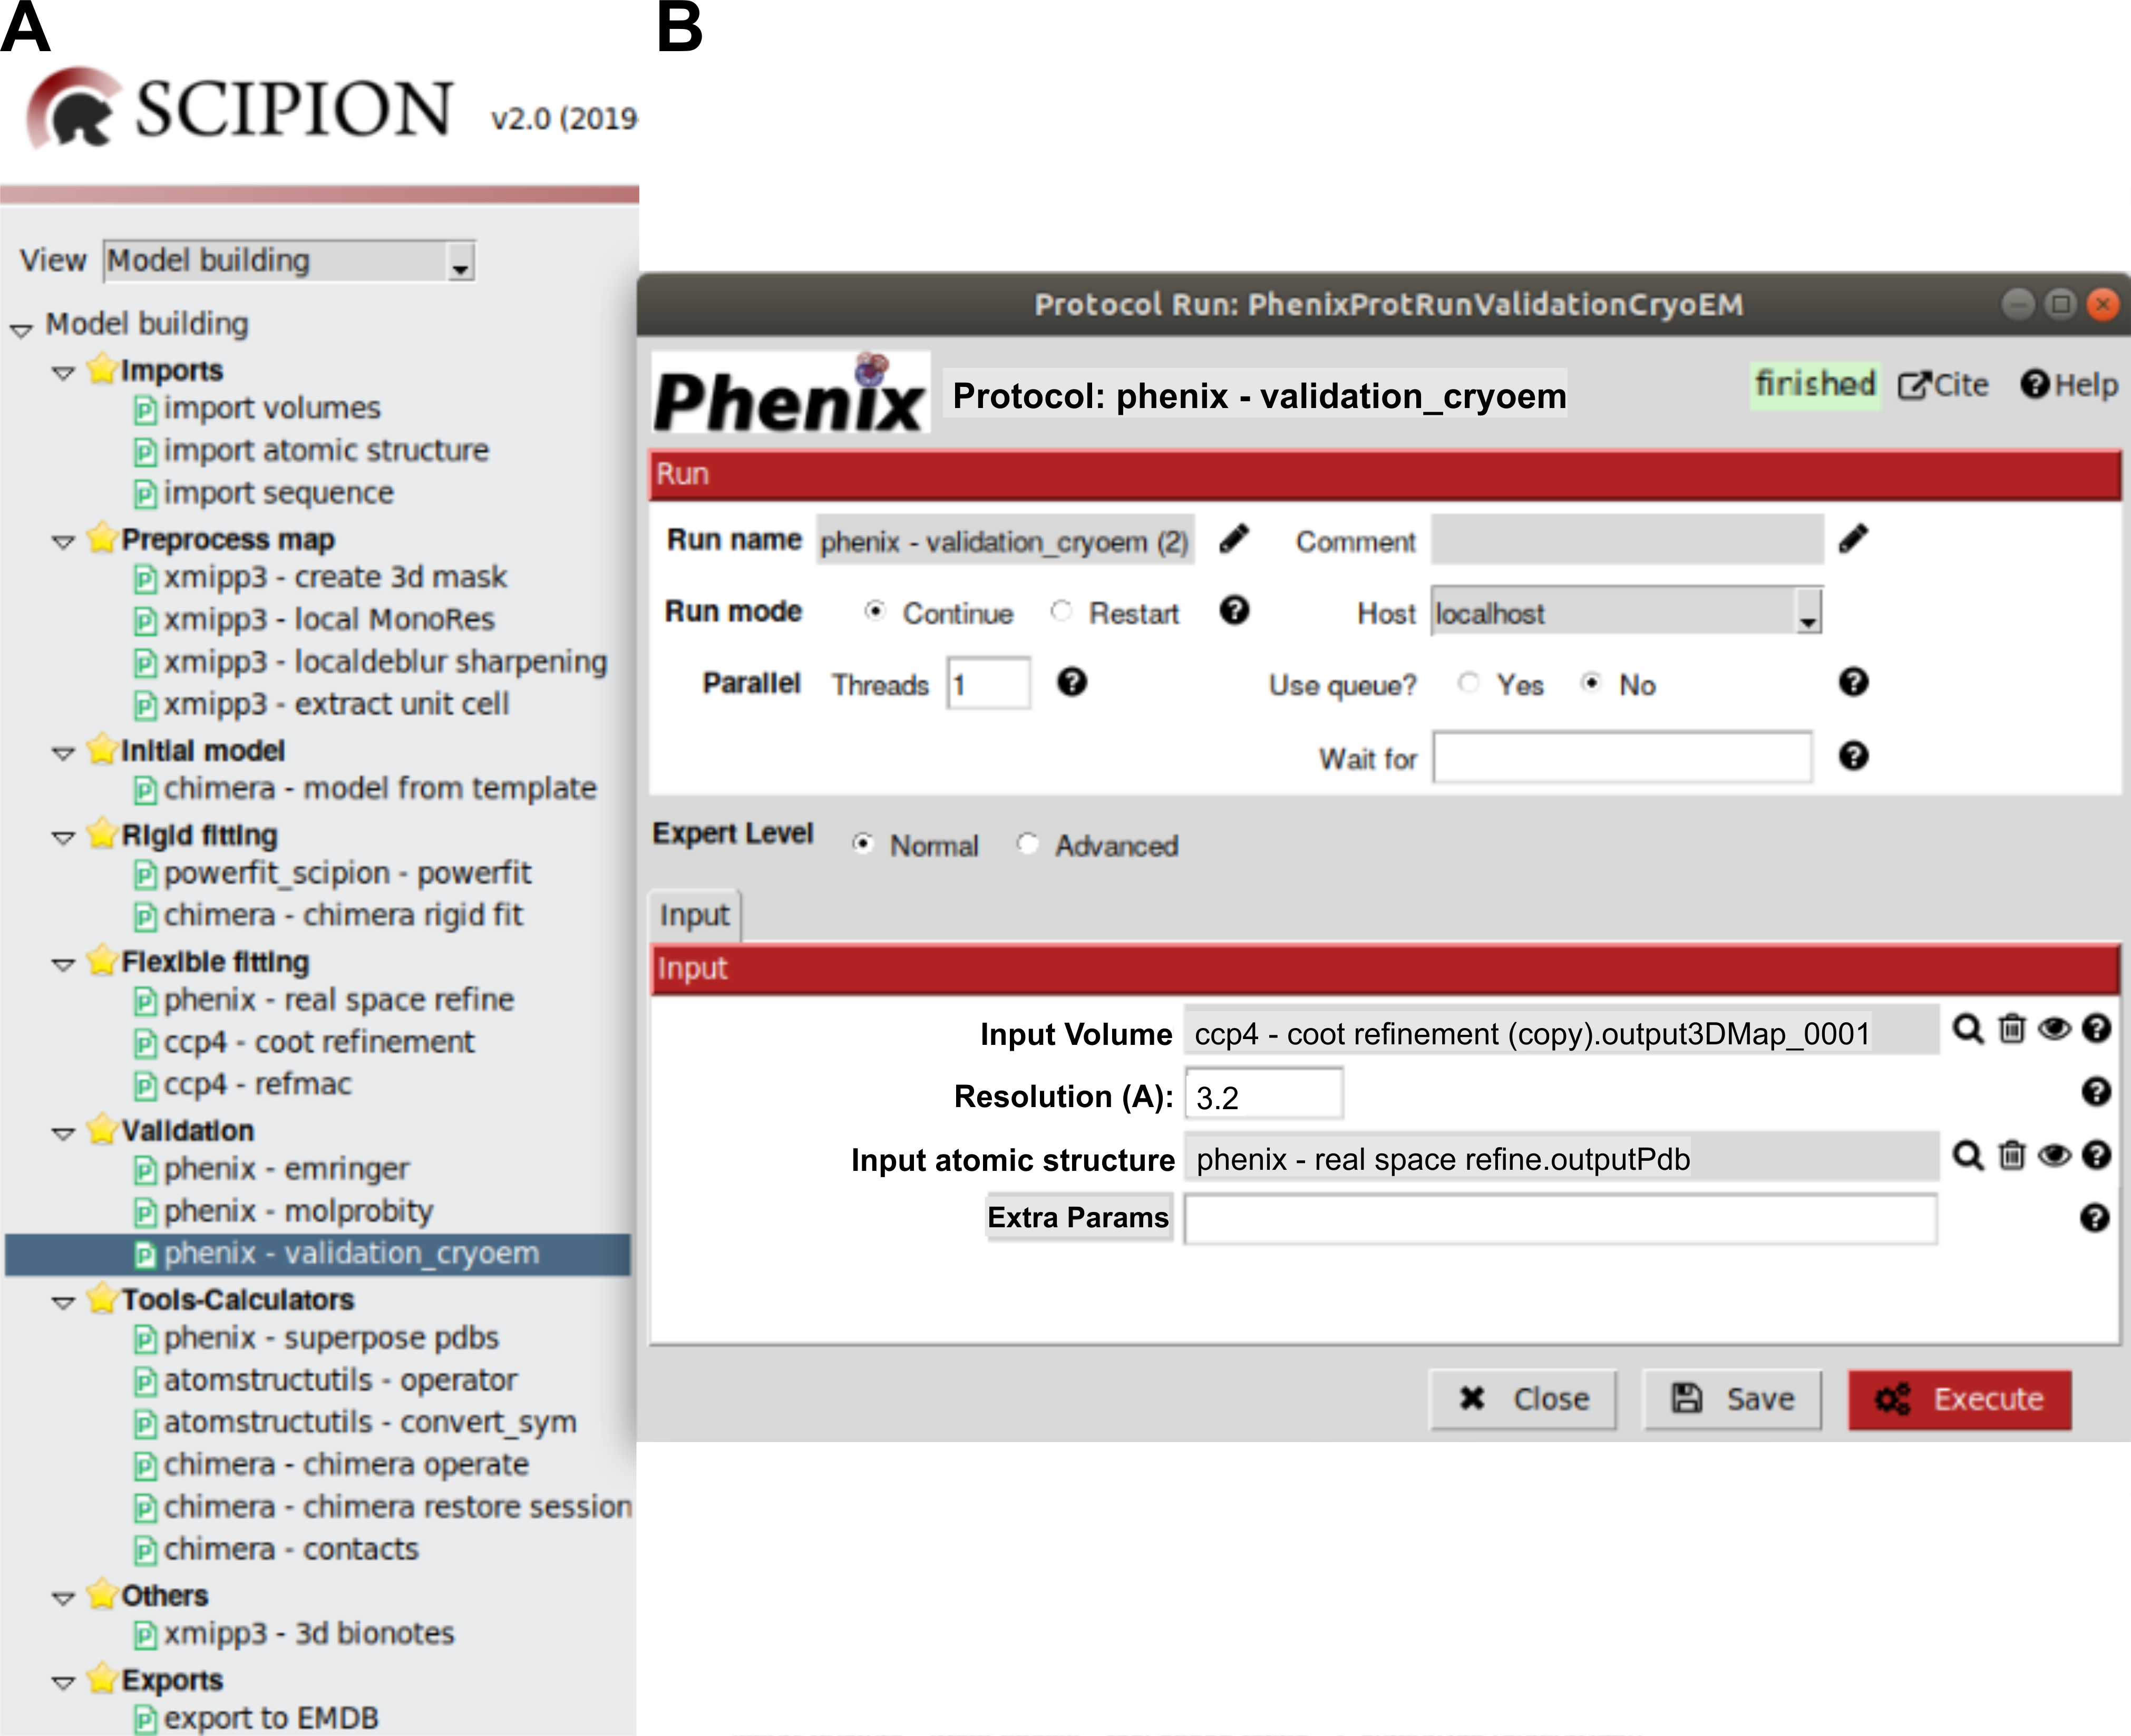
\includegraphics[width=0.90\textwidth]{Images_appendix/Fig157}
     \caption{Protocol \scommand{phenix - validation\_cryoem}. A: Protocol location in \scipion menu. B: Protocol form.}
     \label{fig:validationCryoEM_protocol_1}
    \end{figure}
    
    \begin{itemize}
     \item \ttt{Input Volume}: Electron density map previously downloaded or generated in \scipion.
     \item \ttt{Resolution (\AA)}: \ttt{Input Volume} resolution.
     \item \ttt{Input atomic structure}: Atomic structure previously downloaded or generated in \scipion and fitted to the electron density map.
     \item \ttt{Extra Params}: Advanced param that allows to add a string to the phenix command including other \iii{phenix.real\_space\_refine} program params. Syntax to add extra params: \ttt{paramName1} = \ttt{value1} \ttt{paramName2} = \ttt{value2}
    \end{itemize}
 
 \item Protocol execution:\\
 Adding specific map/structure label is recommended in \ttt{Run name} section, at the form top. To add the label, open the protocol form, press the pencil symbol at the right side of \ttt{Run name} box, complete the label in the new opened window, press OK and, finally, close the protocol. This label will be shown in the output summary content (see below). If you want to run again this protocol, do not forget to set to \ttt{Restart} the \ttt{Run mode}.\\
  Press the \ttt{Execute} red button at the form bottom.
  
 \item Visualization of protocol results:
 
 After executing the protocol, press \ttt{Analyze Results} and the results window will be opened (\ffigure{fig:validationCryoEM_protocol_2}). 
  
    \begin{figure}[H]
     \centering 
     \captionsetup{width=.9\linewidth} 
     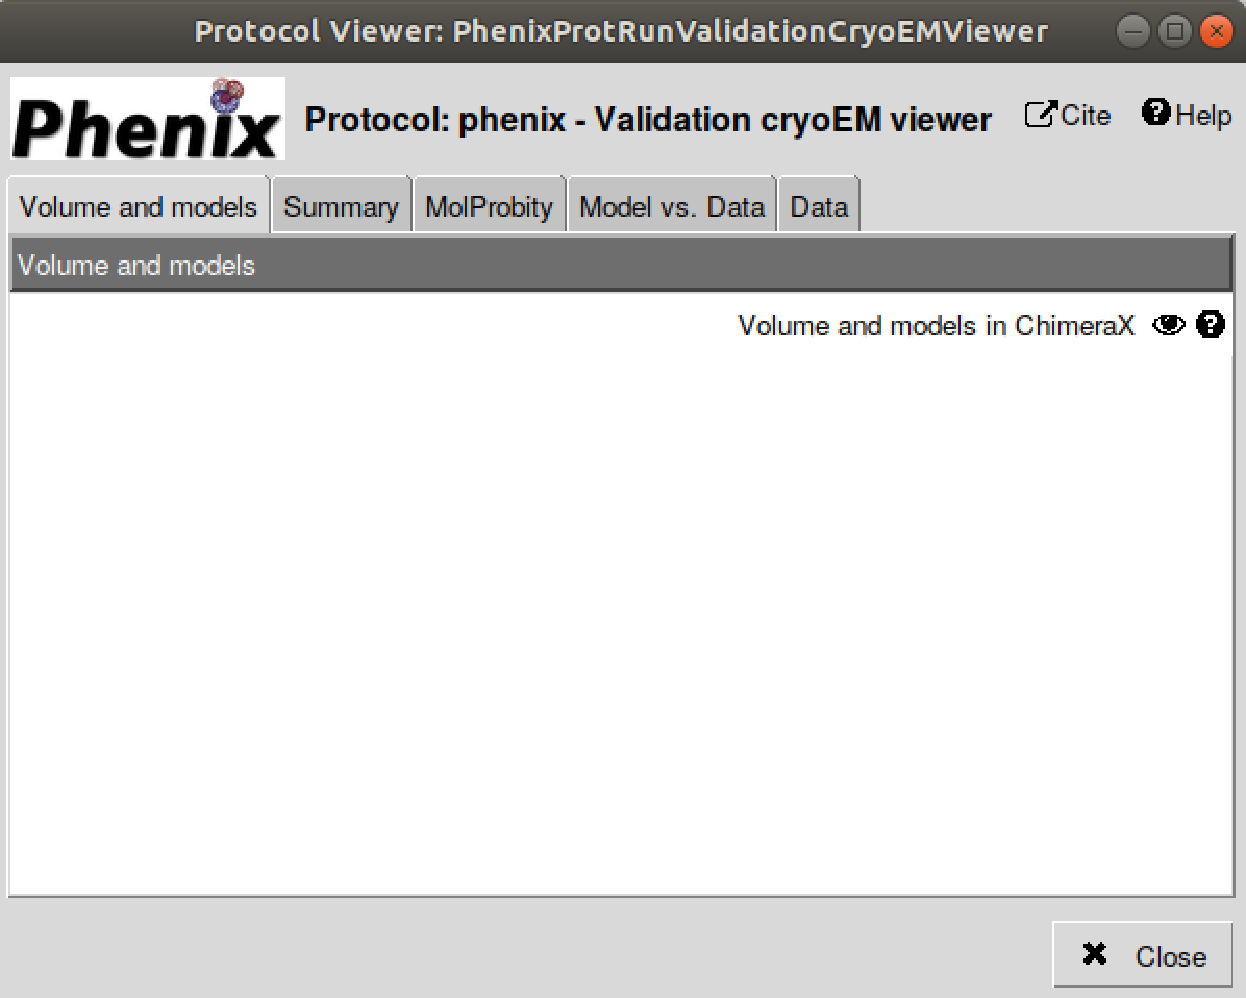
\includegraphics[width=0.50\textwidth]{Images_appendix/Fig200.pdf}
     \caption{Protocol \scommand{phenix - validation\_cryoem}. Taps to visualize \iii{Validation CryoEM} results.}
     \label{fig:validationCryoEM_protocol_2}
    \end{figure}
    
Five taps are shown in the upper part of the results window:
   \begin{itemize}
     \item \ttt{Volume and models}: \chimera graphics window will be opened by default. Atomic structure and volume are referred to the origin of coordinates in \chimera. To show the relative position of atomic structure and electron density volume, the three coordinate axes are represented; X axis (red), Y axis (yellow), and Z axis (blue) (\ffigure{fig:app_protocol_volume_3}).
     \item \ttt{Summary}: Three different summary tables are shown to describe the results obtained from \ttt{Model, Data} and \ttt{Model vs. Data} (\ffigure{fig:validationCryoEM_protocol_3}). Concerning the atomic \ttt{Model}, numeric data from chains, residues, atoms and geometry are described, as well as main \molprobity statistics. \ttt{Data} summarizes experimental map box dimensions and different values of resolution computed with or without a mask. \ttt{Model vs. Data}\ details main real-space correlation coefficients.
        \begin{figure}[H]
         \centering 
         \captionsetup{width=.9\linewidth} 
         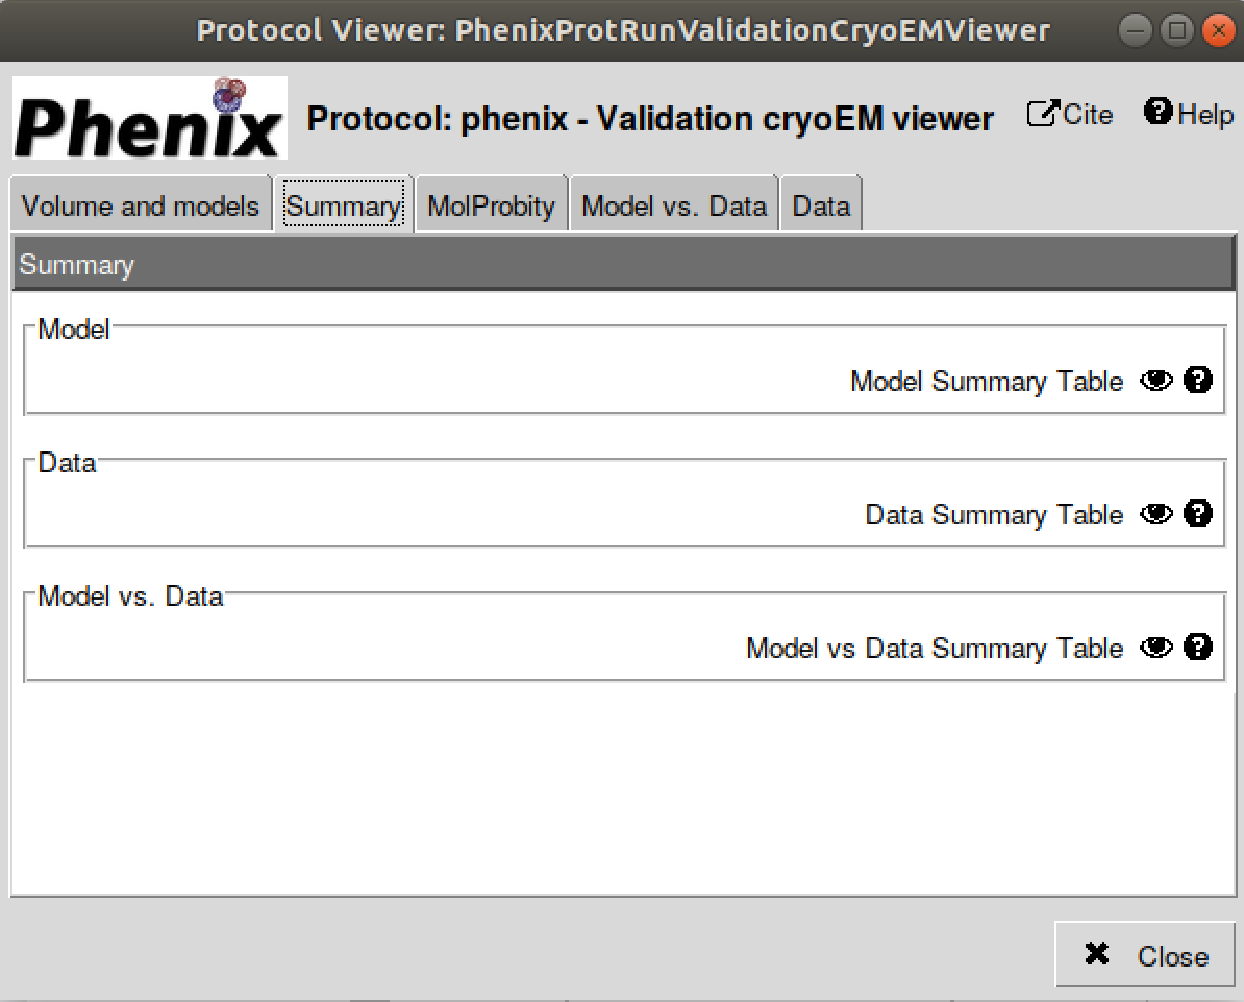
\includegraphics[width=0.50\textwidth]{Images_appendix/Fig201.pdf}
         \caption{Protocol \scommand{phenix - validation\_cryoem}. Summary tables of main\phenix \ttt{validation\_cryoem} results.}
         \label{fig:validationCryoEM_protocol_3}
        \end{figure}
     \item \ttt{MolProbity}: Statistics concerning the atomic model, most of them obtained from \molprobity (\ffigure{fig:validationCryoEM_protocol_4}).
        \begin{figure}[H]
         \centering 
         \captionsetup{width=.9\linewidth} 
         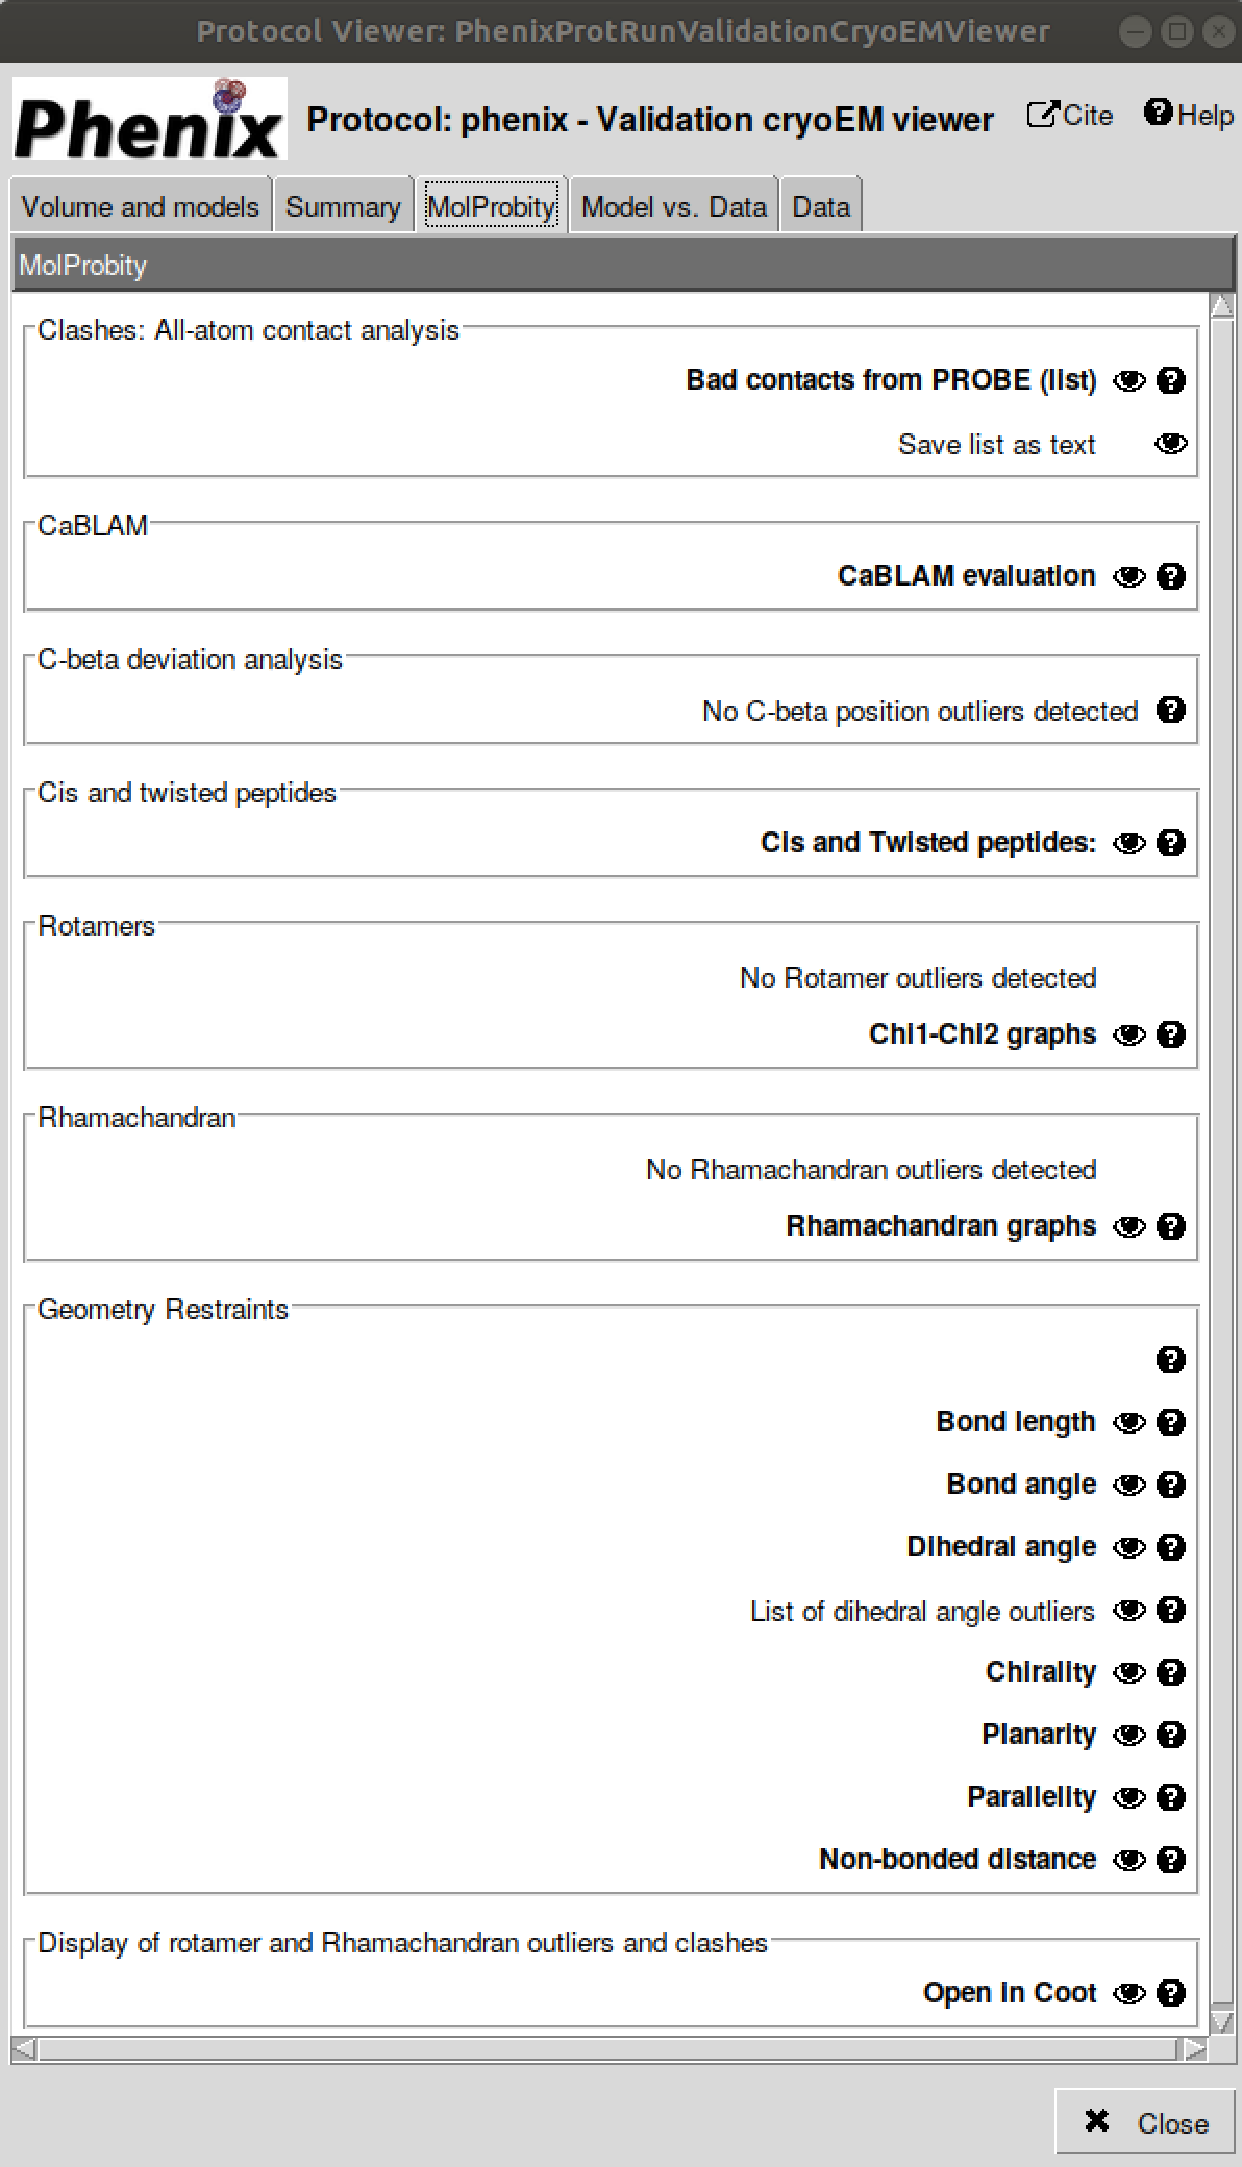
\includegraphics[width=0.50\textwidth]{Images_appendix/Fig202.pdf}
         \caption{Protocol \scommand{phenix - validation\_cryoem}. \molprobity and other statistics of the atomic model.}
         \label{fig:validationCryoEM_protocol_4}
        \end{figure}
        
        \begin{itemize}
         \item \ttt{Clashes: All-atom contact analysis}: List that contains all severe clashes (non-H atoms overlaping more than 0.4 \AA) found by PROBE. All these clashes can be visualized and solved graphically in \coot. If no hydrogens were present, REDUCE adds them before running PROBE. The list can be saved in a folder selected by the user.
         \item \ttt{CaBLAM: C-Alpha Based Low-resolution Annotation Method}: Method designed to assess the mainchain geometry of the atomic model by using protein C\textsubscript{$\alpha$}\xspace geometry and to identify areas of probable secondary structure. Residues that fall outside contours of expected protein behaviour based on high-quality datasets are considered outliers.
         \item \ttt{C-beta deviation analysis}: C\textsubscript{$\beta$}\xspace outliers deviate from ideal positions by more than 0.25\AA. Ideal C\textsubscript{$\beta$}\xspace position is determined from the average of the ideal C-N-CA-CB and N-C-CA-CB dihedrals. This measure is more sensitive than individual measures to both sidechain and mainchain misfittings. Its deviation is an indicator of incompatibility between sidechain and backbone. 
         \item \ttt{Cis and twisted peptides}: Residues showing $cis$ or $twisted$ conformations that could be modeling errors. $cis$ conformations are observed in about 5\% of Prolines and 0.03\% of general residues. Twisted peptides are almost certainly modeling errors.
         \item \ttt{Rotamers}: Rotamer outlier list contains residues that adopt an unusual conformation of $\chi$ dihedral angles. These outliers, commonly used to characterize the conformation of protein sidechains, are detailed in Chi1-Chi2 graph, shown below.
         \item \ttt{Rhamachandran}: Rhamachandran outlier list contains residues that show an unusual combination of their $\phi$ (C-N-CA-C) and $\psi$ (N-CA-C-N) dihedral angles. Most of the time, Ramachandran outliers are a consequence of mistakes during the data processing. These outliers are detailed below in Rhamachandran graphs.
         \item \ttt{Geometry Restraints}: Statistics for geometry restraints used in refinement. Although in general a fully refined structure should not have any outliers, exceptionally there are some of them that are obvious in high resolution electron density maps. Types of restraints:
            \begin{itemize}
             \item \ttt{Bond Length}: This table indicates the number of outliers and the number of restraints (in accordance with the bond length restraints library). The list of outliers details the bonded pairs of atoms sorted by deviation (higher than 4 sigmas).
             \item \ttt{Bond Angle}: This table indicates the number of outliers and the number of restraints (in accordance with the bond angle restraints library). The list of outliers details the bonded triplets of atoms sorted by deviation (higher than 4 sigmas). 
             \item \ttt{Dihedral Angle}: This table indicates the number of outliers and the number of restraints (in accordance with the side chain dihedral torsion - chi- angle restraints library). The list of outliers details the bonded tetrads of atoms sorted by deviation (higher than 4 sigmas).
             \item \ttt{Chilarity}: This table indicates the number of restraints (in accordance with the volume chilarity restraints library).
             \item \ttt{Planarity}: This table indicates the number of restraints (in accordance with the volume planarity restraints library).
             \item \ttt{Parallelity}: This table indicates the number of restraints (in accordance with the volume parallelity restraints library).
             \item \ttt{Non-bonded distance}: This table indicates the number of restraints (in accordance with the volume non-bonded distance restraints library).
            \end{itemize}
         \item \ttt{Display of rotamer and Rhamachandran outliers and clashes}: Interactive visualization of outliers (Ramachandran, rotamer and C\textsubscript{$\beta$}\xspace) and severe clashes with \coot.
        \end{itemize}
      \item \ttt{Model vs. Data}: Real-space correlation coefficients between map and model-derived map (\ffigure{fig:validationCryoEM_protocol_5}).
       \begin{figure}[H]
         \centering 
         \captionsetup{width=.9\linewidth} 
         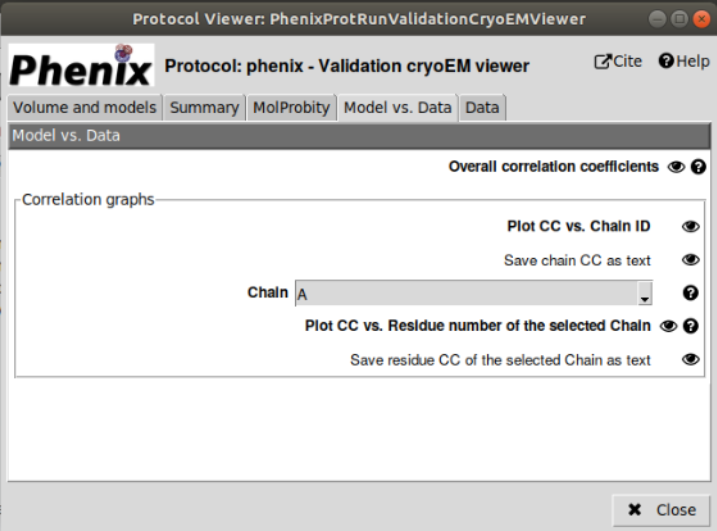
\includegraphics[width=0.50\textwidth]{Images_appendix/Fig203.pdf}
         \caption{Protocol \scommand{phenix - validation\_cryoem}. Real-space correlation results.}
         \label{fig:validationCryoEM_protocol_5}
        \end{figure}
        \begin{itemize}
         \item \ttt{Overall correlation coefficients} \citep{afonine2018b}: 
         \begin{itemize}  
          \item \ttt{Mask CC}: Correlation coefficient between the model-derived map and the experimental map inside the mask region built around the model with a fixed radius. This comparison aims to fit the atomic centers.
          \item \ttt{Box CC}: Correlation coefficient between the model-derived map and the whole experimental map. This comparison aims to assess the similarity of maps and remark map densities that have not been modeled.
          \item \ttt{Volume CC}: Correlation coefficient between the model-derived map and the experimental map inside the mask region built around the model considering only model-derived map regions with the highest density values, ignoring regions below a certain contouring density threshold. Particularly, in this case the N points with the highest density, inside the molecular mask, are taken into account. This comparison aims to fit the molecular envelope defined by the model-derived map.
          \item \ttt{Peak CC}: Correlation coefficient between the model-derived map and the experimental map that considers only map regions with the highest density values, ignoring regions below a certain contouring density threshold. Particularly, in this case the N points with the highest density, simultaneously present in the model-calculated map and in the experimental map, are taken into account. This comparison aims to fit the strongest peaks in model-derived and experimental maps.
          \item \ttt{Main chain CC}
          \item \ttt{Side chain CC}
         \end{itemize}
         \item \ttt{Correlation graphs}:
         \begin{itemize}
           \item \ttt{Plot CC vs. Chain ID}: Plot of correlation coefficients regarding the chain IDs. These correlation coefficient values can be saved in a text file in the folder selected by the user.
           \item \ttt{Plot CC vs. Residue number of the selected Chain}: Plot of correlation coefficients of each chain residues. The specific chain is selected by the user in the chain option box. These correlation coefficient values for each chain can be saved in a text file in the folder selected by the user.
         \end{itemize}
        \end{itemize}
      \item \ttt{Data} (\ffigure{fig:validationCryoEM_protocol_6}): Computation of Resolution  and FSC.
       \begin{figure}[H]
         \centering 
         \captionsetup{width=.9\linewidth} 
         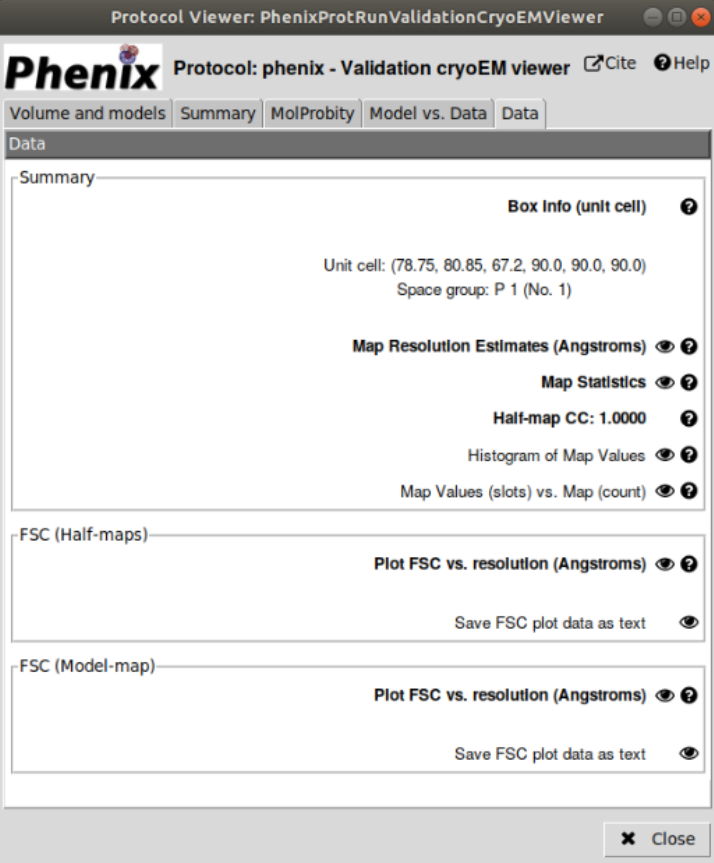
\includegraphics[width=0.50\textwidth]{Images_appendix/Fig204.pdf}
         \caption{Protocol \scommand{phenix - validation\_cryoem}. Experimental data results.}
         \label{fig:validationCryoEM_protocol_6}
        \end{figure}
        \begin{itemize}
         \item \ttt{Summary}: Basic statistics about the maps and summary of resolution estimates.
         \begin{itemize}
          \item \ttt{Box info (unit cell)}: Map cell dimensions (pixels).
          \item \ttt{Map Resolution Estimates (Angstroms)}: Resolution estimates computed considering both map experimental data and model-derived information(with and without mask)\setlength{\parindent}{12pt}.\\
            \ttt{- Using map alone (d99)}: Resolution cutoff beyond which Fourier map coefficients are negligibly small. Calculated from the full map or from each one of half maps [d99 (half map 1), d99 (half map 2)].\\
            \ttt{- Overall Biso}: Overall isotropic B-value.\\
            \ttt{- d\_model}: Resolution cutoff at which the model map is the most similar to the target (experimental) map. Requires map and model. For d\_model to be meaningful, model is expected to fit the map as well as possible. \\
            \ttt{- d\_model (B factors = 0)}: It tries to avoid the blurring of the map.\\
            \ttt{- FSC (model) = 0}: d\_FSC\_model\_0; Resolution cutoff up to which the model and map Fourier coefficients are similar at FSC value 0.\\
            \ttt{- FSC (model) = 0.143}: d\_FSC\_model\_0.143; Resolution cutoff up to which the model and map Fourier coefficients are similar at FSC value 0.143.\\
            \ttt{- FSC (model) = 0.5}: d\_FSC\_model\_0.5; Resolution cutoff up to which the model and map Fourier coefficients are similar at FSC value 0.5.\\
            \ttt{- FSC (half map 1, 2) = 0.143}: d\_FSC; Highest resolution at which the experimental data are confident. Obtained from FSC curve calculated using two half-maps and taken at FSC=0.143. The two half maps are required to compute this value.\\
            \ttt{- Mask smoothing radius (Angstroms)}: Radius of the default soft mask used since sharp edges resulting from applying a binary mask may introduce Fourier artifacts.\\
         \end{itemize}
         \item Fourier shell correlation taps:
          \begin{itemize}
           \item \ttt{FSC(Half-maps)} (Only if two half maps have been added as inputs): FSC plot regarding the resolution (\AA) and the spatial frequency (1/\AA) based on half maps with and without masking. The intersections of the curves with FSC = 0.143 are shown. FSC plot data can be saved as text file in a folder selected by the user.
           \item \ttt{FSC (Model-map)}: FSC plot regarding the resolution (\AA) and the spatial frequency (1/\AA) based on the experimental map and the model-derived map with and without masking. The intersections of the curves with FSC = 0.5 are shown. FSC plot data can be saved as text file in a folder selected by the user.
          \end{itemize}
        \end{itemize}
    \end{itemize}
    
 \item Summary content:\\
    \ttt{Protocol output}: Empty.\\
    \ttt{SUMMARY} box:\\Main $MolProbity$ statistics computed by the $Phenix$ package to assess protein geometry using the same distributions as the MolProbity server:
      \begin{itemize}     
        \item \ttt{Ramachandran outliers}: Percentage of residues assessed that show an unusual combination of their $\phi$ (C-N-CA-C) and $\psi$ (N-CA-C-N) dihedral angles.
        \item \ttt{Ramachandran favored}: Percentage of residues assessed that show an normal combination of their $\phi$ (C-N-CA-C) and $\psi$ (N-CA-C-N) dihedral angles. Ramachandran outliers and favored residues are detailed in the \ttt{Ramachandran plot}. Allowed residues are included in the small region comprised between the favored and the outlier region.
        \item \ttt{Rotamer outliers}: Percentage of residues assessed that adopt an unusual conformation of $\chi$ dihedral angles. Rotamer outliers, commonly used to characterize the conformation of protein sidechains, are detailed in Chi1-Chi2 plot.
        \item \ttt{C-beta outliers}: Number of residues showing an unusual deviation (higher than 0.25 \AA) of the C{$\beta$} from its ideal position. This deviation is an indicator of incompatibility between sidechain and backbone. 
        \item \ttt{Clahscore}: Score associated to the number of pairs of non-bonded atoms unsually close to each other, showing probable steric overlaps. Clashscore is calculated as the number of serious clashes per 1000 atoms. This value has to be as low as possible.
        \item \ttt{Overall score}: $MolProbity$ overall score representing the experimental resolution expected for the structure model. This value should be lower than the actual resolution. The lower the value, the better quality of the structure model.
      \end{itemize}

\end{itemize}
